\documentclass[letterpaper,twocolumn,amsmath,amssymb,pre]{revtex4-1}
\usepackage{graphicx}% Include figure files
\usepackage{color}

\newcommand{\red}[1]{{\bf \color{red} #1}}
\newcommand{\blue}[1]{{\bf \color{blue} #1}}
\newcommand{\green}[1]{{\bf \color{green} #1}}

\newcommand{\fixme}[1]{\red{[#1]}}
\newcommand{\davidsays}[1]{{\color{red} [\green{David:} \emph{#1}]}}
\newcommand{\renesays}[1]{{\color{red} [\blue{Rene:} \emph{#1}]}}
\newcommand{\jeffsays}[1]{{\color{red} [\blue{Jeff:} \emph{#1}]}}

\newcommand\micron{\ensuremath{\mu\text{m}}}

\begin{document}
\title{Robustness of MinD oscillation in \emph{Escherichia coli} with
  diverse cell shapes}

\author{Jeff B. Schulte}
\affiliation{Department of Physics, Oregon State University}
\author{Rene W. Zeto}
\affiliation{Department of Physics, Oregon State University}
\author{David Roundy}
\affiliation{Department of Physics, Oregon State University}

\begin{abstract}
  The dynamics of the Min-protein system help Escherichia coli
  bacteria regulate the process of cell division by identifying the
  center of the cell.  We model the Min-protein system in bacteria
  that have been forced into unusual flattened shapes, as have
  recently been experimentally observed.  We find that although the
  presence of Min oscillations is robust in a wide variety of cellular
  configurations, the location of the peaks is strongly affected by
  the cellular shape.  In some cases no periodic oscillations are
  observed.  In particular, we find that cellular shapes observed
  experimentally to present irregular oscillations do so in the
  theoretical model, consistently \fixme{or inconsistently?} with
  experiment.  \fixme{In agreement with previous theoretical and
    experimental results, we observe ``rotating'' behavior in certain
    shapes having three corners.}
\end{abstract}

\maketitle

\section{Introduction}
\fixme{Huang and those who reference him use the terms 'numerical
  deterministic reaction-diffusion model' and 'stochastic version of
  this model' for the stochastic.} It is vital that during the process
of bacterial cell division a cell avoid minicelling, or splitting into
daughter cells with lopsided volumes.  Instrumental to this process in
\emph{Escherichia coli} is a long FtsZ polymer chain that develops on
the cell wall in the center region of the cell, helping dictate the
plane of
division~\cite{adams2009bacterial,lutkenhaus2007assembly}. Previous
experimental studies have shown that the MinC protein, known to
inhibit the FtZ polymer\cite{shen2010examination}, exhibits regular
pole to pole oscillatory behavior between both ends of the wild-type
pill-shaped cell.  It thus has a higher time averaged concentration in
the cell poles than in the center region, which aides in prohibiting
the FtZ from developing in the wrong region.  The MinC is recruited to
these poles by MinD, which ineracts with another protein, MinE, that
is neccesary for MinD
oscillation.~\cite{hu1999topological,fu2001mine,shapiro2009and,yu1999ftsz,raskin1999rapid,meacci2005min,raskin1999minde}.

Previous studies have shown that the minD protein system is capable of
exhibiting oscillations in round shapes \cite{fange2006noise}as well
as in connected three pronged tube shapes~\cite{varma2008min}, in
which the oscillations seem to seek out the extreme poles in the
cell~\cite{corbin2002exploring,juarez2010changes}.

However, Mannik \emph{et al.} have also shown that there are
limitations to this robust capability to
oscillate~\cite{mannik2010bacteria,mannik2009bacterial}. They have
experimentally forced E. Coli cells into silicon microfabricated
channels of $0.25\micron$ thickness. Upon entering the channels, the
cells undergo a rapid mechanical deformation in which they widen along
their short axis parallel to the channel plane, followed by a slower,
broadening out along both free axes.  This deformation results in very
wide (they can reach widths of over $5\micron$), flattened cells that
when view from the top down show very irregular and assymetric shapes.
While these cells are still able to divide into surprisingly equal
volumes, the MinD oscillations within lose their regularity, both
temporally and spatially. Seen with flourescent microscopy (after
using common genetic techniques to allow the cells to flouresce), the
MinD seem to maximize in multiple locations within the cell, in a
seemingly random sequence. This allows for an opportunity to test
previously studied MinD simulation models against more extreme
experimental cases than have been seen thus far. \fixme{Perhaps this
  sentence should come later after we've introduced the simulation
  research that's been done.}

A significant amount of work has been done to develop protein reaction
and diffusion simulation models that exhibit accurate macroscopic
dynamics of the MinD protein system. Early models involve free
proteins that affect each others' rates of diffusion and membrane
attachment, but do not combine into compound
states~\cite{meinhardt2001pattern}.  In 2003 Huang improved upon this
work with a simple and very successful simulation model based on
MinD-MinE combination, ATPase hydrolysis, and MinD membrane attachment
that exhibits accurate MinD oscillations in cylindrical
cells~\cite{huang2003dynamic}. In this model cytoplasmic MinD is more
likely to attach to the membrane when MinD is already clustered there
(following observed non-linear attachement of minD on the cell
membrane), and is stationary once attached.  A number of studies have
used an approach similar in that they do not rely on the ability of
MinD to move along the walls and
cluster~\cite{kruse2007experimentalist, meinhardt2001pattern,
  drew2005polymerization, fange2006noise, kerr2006division}, while
studies have been made as well of models which rely on MinD mobility
and attraction on the cell membrane~\cite{kruse2002dynamic,
  howard2005cellular}.  Experimental studies of the Min system's
association with the cell membrane have also been
made~\cite{hsieh2010direct,mileykovskaya2003effects}.

Variations of the Huang 2003 model that stochasticly account for
molecular interaction and diffusion~\cite{fange2006noise} and
monte-carlo simulations that implement this stochastic version of
Huang's mean field reaction rates~\cite{kerr2006division} broadly
confirm the major results obtained by Huang's model.  However, they
more successfully predict experimentally observed oscillations in
round cell phenotypes~\cite{fange2006noise, huang2004min} and
variations in other
quantities~\cite{kruse2007experimentalist}\fixme{If going to use this
  sentence should list these and reference properly?}. Both
deterministic and stochastic models are widely used throughout systems
biology~\cite{lawson2013spatial,robb2014stochastic,oguz2014stochastic,fu2013deterministic,rudiger2014stochastic},
and it's important to better understand their limitations.  Manniks'
experiments allow for a new distinct opportunity to test these two
approaches further.
%% Biochemical models of broader scope have also been
%% used to study the MinD system and show consistent
%% results~\cite{arjunan2010new}.

%% \fixme{There are not any direct comparisons of the deterministic and
%%   stochastic models that I can find other than the fange2006 paper
%%   cited above for the round cells.  Those showed that the
%%   deterministic sims are 'bistable' - one type of initial conditions
%%   (MinD starting on walls on one side) show oscillations, another type
%%   (half cyto is filled with 3/4 of MinD) don't.  Huang in 2004 paper
%%   cited above uses numerical determinisitc and finds that it can show
%%   oscillations in round cells as well, but right now I can't find it
%%   and the journal doesn't give me access to it.  predict oscillations
%%   in perfectly round cells unless noise was added to the simulation,
%%   but could in almost round ellipses.  It seems that once the
%%   stochastic models began to be used, nobody really used the
%%   deterministic model any longer.  Not sure what to say about this in
%%   order to introduce what we do here properly.}

In this paper we apply a deterministic model and a stochastic model
of simulation and compare them against Mannik's experimental findings.


\fixme{Following paragraph is awkward, and I don't think it's needed.}
Studies have shown as well that MinD binds preferentially to regions
enriched with cadiolipin, an anionic phospholipid that collects on
regions of high negative curvature. This mechanism has been
incorporated into other
models.\cite{drew2005polymerization,cytrynbaum2007multistranded,renner2012mind,renner2012mind}
However, this mechanism of combined clustering, phospholipids and MinD
has not been observed in real cells. \cite{halatek2012highly}


\begin{figure}
  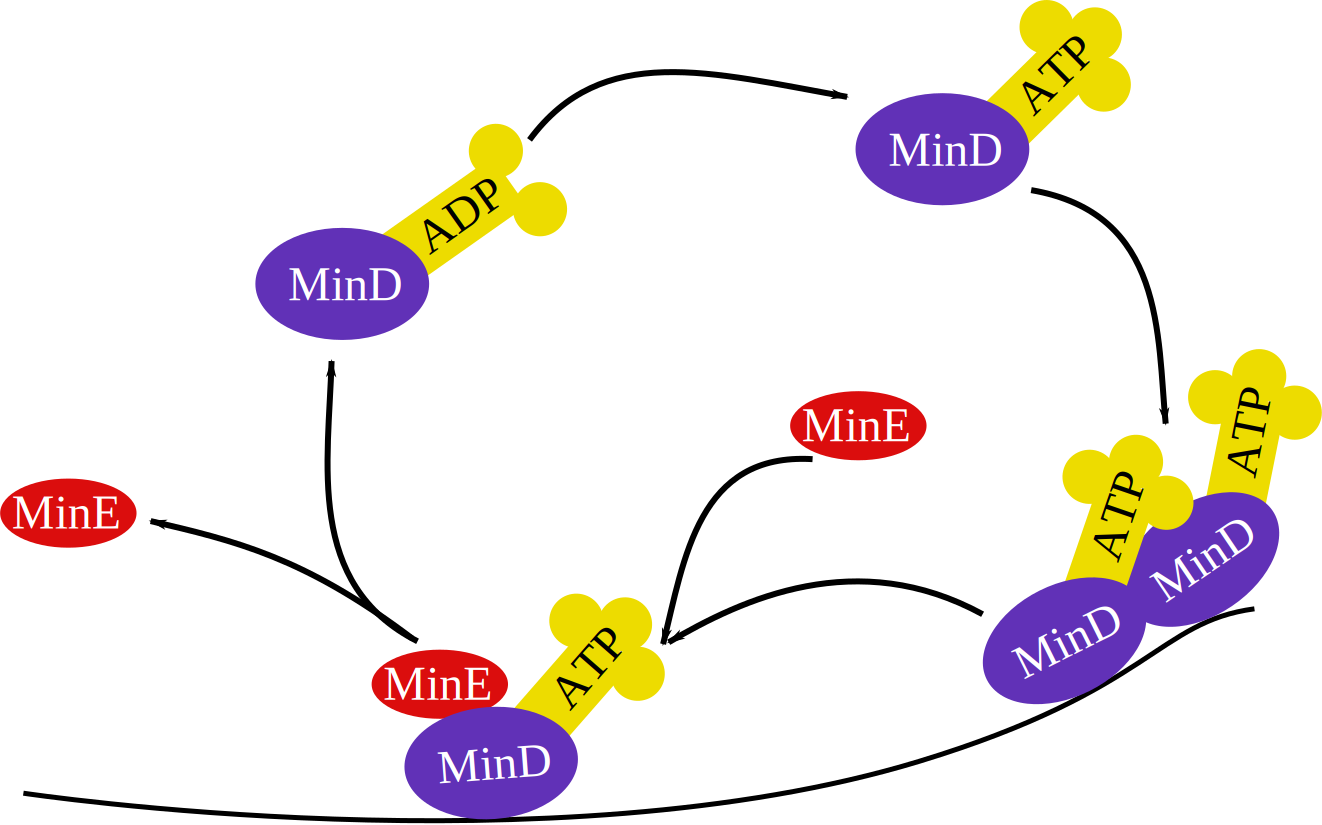
\includegraphics[width=\columnwidth]{reactions}
  \caption{Reactions included in the model of Huang \emph{et
      al.}~\cite{huang2003dynamic}.}\label{fig:reactions}
\end{figure}


\section{Model, Methods, and Cell Shapes}\label{sec:model-method-shapes}
We implement the reaction-diffusion model of Huang \emph{et
  al.}~\cite{huang2003dynamic}.  Figure~\ref{fig:reactions} shows the
reaction process.  The cytoplasmic MinD:ADP complex undergoes
nucleotide exchange and is changed into the MinD:ATP complex.  This
will naturally diffuse and attach to the cell membrane.  A cytoplasmic
MinE will attach to the wall bound MinD:ATP complex and after a time
will activate ATP hydrolosis.  This breaks up the complex, releasing
MinE, phosphate, and MinD:ADP back into the cytoplasm.  The MinD:ADP
will undergo nucleotide exchange and begin again the cyclic process.
The model is defined by a set of five reaction-diffusion equations:

\begin{multline}
  \frac{\partial \rho_{D:ADP}}{\partial t} = \mathcal{D}_D\nabla^2\rho_{D:ADP}-k_D^{ADP\rightarrow ATP}\rho_{D:ADP}\\
  +\delta(d_w)k_{de}\sigma_{DE},\hspace{3.4cm}
\end{multline}
\begin{multline}
  \frac{\partial \rho_{D:ATP}}{\partial t} = \mathcal{D}_D\nabla^2\rho_{D:ATP}+k_D^{ADP\rightarrow ATP}\rho_{D:ADP}\\
  -\delta(d_w)[k_D+k_{dD}(\sigma_D+\sigma_{DE})]\rho_{D:ATP}
\end{multline}
\begin{multline}
  \frac{\partial \rho_E}{\partial t} = \mathcal{D}_E\nabla^2\rho_E+\delta(d_w)k_{de}\sigma_{DE}
  -\delta(d_w)k_E \sigma_D \rho_E
\end{multline}
\begin{multline}
  \frac{\partial \sigma_D}{\partial t} = -k_E\sigma_D\rho_E
  +[k_D+k_{dD}(\sigma_D+\sigma_{DE})]\rho_{D:ATP}
  \label{eq:d-on-wall}
\end{multline}
\begin{multline}
  \frac{\partial \sigma_{DE}}{\partial t} = -k_{de}\sigma_{DE}+k_E\sigma_D\rho_E\hspace{3cm}
  \label{eq:FifthPDE}
\end{multline}
where $\rho$ is cytoplasmic protein density ($\micron^{-3}$), $\sigma$
is membrane bound density ($\micron^{-2}$), $\mathcal{D}_D$ and
$\mathcal{D}_{E}$ th diffusions constants for MinD and MinE,
respectively, $k_D^{\textrm{ADP $\rightarrow$ ATP}}$ the rate of
conversion from MinD:ADP to the MinD:ATP complex, $k_D$ the rate of
MinD:ATP attachement to the membrane when no protein is already
attached there, $k_{dD}$ the increase of this rate when MinD:ATP is
present on the membrane, $k_{de}$ the rate of hydrolisis of the
MinD:MinE:ATP complex, $k_E$ the rate of cytoplasmic MinE binding to
membrane bound MinD:ATP complex, and $d_w$ is the distance from the
point in space to the closest wall.  The Dirac delta function
$\delta(d_w)$ has units of $\micron^{-1}$ and is zero everywhere except
at the wall.  Equations \ref{eq:d-on-wall} and \ref{eq:FifthPDE} are
only relevent at the membrane because the membrane-bound density
values have no meaning in the cytoplasm.

Our diffusion and reaction rates are shown below.  We are interested
primarily in the effect of cellular size and shape on the protein
oscillations, so we follow Huang\cite{huang2003dynamic} and do not
deviate from the wild type values used in the cited work.

\begin{gather*}
  \mathcal{D}_D = \mathcal{D}_{E} = 2.5\micron^2/\text{sec}\\
  k_D^{\textrm{ADP $\rightarrow$ ATP}} = 1/\textrm{sec,  }
  k_D = 0.025 \micron /\textrm{sec}\\
  k_{dD} = 0.0015 \micron^3/ \textrm{sec,  }
  k_{de} = 0.7/\textrm{sec}\\
  k_E = 0.093 \micron^3 /\textrm{sec}.
\end{gather*}

Huang's simulations use total MinD and MinE concentrations of
$1,000/\micron$ and $350/\micron$, respectively, in a cylindrical cell of
radius $0.5\micron$, and in our (non-cylindrical) cells we use the same
number of proteins per unit volume.  These concentration values are
$1273\micron^{-3}$ and $446\micron^{-3}$, respectively. \fixme{It's been
  a while so might want to check this to make sure it's true.}  We
construct a 3D grid in cartesian coordinates, with a grid spacing of
.05\micron.

We have performed both a basic finite analysis, numerical,
deterministic model simulation that is spatially and temporally
discrete, and a stochastic analysis that is spatially discrete but
continuous in time.  Our stochastic model follows the work of
Kraus~\cite{kraus1996crosstalk} which in turn follows a method
introduced by Gillespie~\cite{gillespie1977exact}.

We mean to investigate the geometric limits of the Min system
oscillations as observed by Mannik \emph{et
  al.}~\cite{mannik2012robustness}, so we model the Min system in
several cell shapes and sizes.  Here we present a selection of these,
beginning with naturally occuring pill-shaped cells, followed by a
number of flattened out shapes which reflect the experiments of Mannik
\emph{et al.}, in which bacteria are confined within a thin slit of
height $0.25\micron$ ~\cite{mannik2012robustness}.  Viewed from the
top down the cells have the shapes described below and viewed from the
side they have at their edges a semicircular protrusion (one may
imagine the shape of a pancake).
%
In this paper we focus on four specific flattened cell shapes.  Two of
these shapes replicate those published by Mannik, and the other two
are `stadium' shapes that respectively have the same aspect ratio,
thickness, and volume as the two Mannik shapes.  Viewed from the top
down, these stadium shapes appear as rectangles with semi-circular end
caps on the long axis ends.

%% Our pill shapes differ from those of Huang \emph{et al.} in that they
%% are cylinders with hemisphere endcaps instead of pure cylindrical
%% shapes.  Our cylinderidrical radius is $0.5\micron$ and the lengths
%% of our cells (measured between the tips of the endcaps) are
%% $5\micron$, $4\micron$, $3\micron$, and $2.5\micron$.

%% \fixme{Is the following Kubitscheck paragraph needed?}
%% Kubitschek has shown in multiple experiments that at the time of cell
%% division cells have a volume that is within a range of roughly
%% $1\micron^3$ to $2\micron^3$~\cite{kubitschek1990cell,
%%   kubitschek1968linear}.  We follow Huang's
%% simulations\cite{huang2003dynamic} and Mannik's experiments and model
%% cells that are slightly larger than this range.

\begin{figure*}
  %\includegraphics[width=\textwidth]{../data/shape-p/3_00-0_50-0_00-0_00-15_00-exact/plots/image-plot}
  \begin{center}
    \includegraphics[width=0.8\textwidth]{../data/shape-p/3_00-0_50-0_00-0_00-15_00-exact/plots/single-image-plot}\\
    \vspace{-2.5em}
    \includegraphics[width=0.8\textwidth]{../data/shape-p/3_00-0_50-0_00-0_00-15_00-full_array/plots/single-image-plot}
    \vspace{-3em}
  \end{center}
  \caption{Contour plot images of the concentration of each protein
    species in a natural pill-shaped bacterium at regular intervals in
    time (one second intervals), with darker regions indicating higher
    concentration. The upper plots shows results from the
    deterministic model and the lower shows results from the
    stochastic model.  The cells pictured are $4\micron$ in length,
    measured from end to end.  The order of frames is such that
    individual MinD proteins begin at the bottom of the plot (in the
    MinD:ATP state in the cytoplasm), and progress upward until they
    reach the MinE:MinD:ATP membrane-bound complex.  At that point,
    they will spontaneously dissociate into cytoplasmic MinE (the top
    row) and the starting state of cytoplasmic MinD:ADP.  The
    densities plotted are integrated along the axis orthogonal to the
    page.  The stochastic densities are broadened using the gaussian
    smearing approach of Zhang \emph{et
      al.}~\cite{zhang2007gaussian}}.
  \label{image-p}
\end{figure*}

Huang \emph{et al}~\cite{huang2003dynamic} has performed a linear
stability analysis on the model which shows an upper limit on a steady
state solution of a $2\micron$ wavelength.  Cells with dimensions longer
than this show spontaneous oscillatory behavoir in this
direction, while cells that are shorter relax into a motionless steady
state.  We have similarly performed a stability analysis in an
infinite slab with a thickness equal to that of our flattened cells
($0.25\micron$) and have found that an equivalent stability limit for
half wavelength is $2.13\micron$. As expected, when decreasing the
lengths and widths of our simulated flattened cells so that the
longest distance across the cell is less than this length, the cells
stop exhibiting any oscillatory behavior.  The deterministic model
relaxes into a motionless state and the stochastic model exhibits
random fluctuations without spatial oscillations.

\fixme{WHERE TO SAY??? : I think we should describe the ``starry
  night'' effect in the stochastic model.}

\section{Naturally Occuring Pill Shaped Cells}

We begin with the naturally occuring pill cell shape.  We peice this
shape together as two hemispherical endcaps attached on either end of
a cylinder.  This shape follows the early simulations of Huang
\emph{et al.} but differs in that we have added the end caps for a
more natural shape, expecting similar results.

Figure~\ref{image-p} shows a series of color plots of protein cycle
stage concentration for both the deterministic and stochastic
models. The cells shown are $4\micron$ in length, measured from end to
end.  We have 'smeared out' the stochastic concentrations in a manner
meant to reproduce the images shown by diffraction limited
flourescence microscopy.  We do so using the two dimensional gaussian
approximation developed by Zhang \emph{et
  al.}~\cite{zhang2007gaussian}.  In this approximation we use a
numerical aperture value of 1.3, which is the same as used by Mannik
experimentally, and a wavelength of $650nm$.  Each frame is 2.5
seconds ahead of the last, and each image shows the concentration of a
given state of protein (of the five described in the reaction model)
summed over the coordinate orthogonal to the page.

Figure~\ref{image-p} begins about 300 seconds into the simulation and
shows one period of oscillation.  At $t=0$ there is a high
concentration of MinD:ATP that has accumulated on the membrane in the
lower section of the cell. An important aspect of Huang's model is
that the MinD is attracted to and sticks to the membrane nonlinearly:
as it accumulates there it begins to 'recruit' other MinD that is
diffusing in the cytoplasm nearby, causing peaks in concentration to
build up on the walls.  Meanwhile, the MinE is creeping downward as it
reacts with the membrane-bound MinD, forming the MinD:MinE:ATP
complex, breaks it apart, and then diffuses downward a bit more before
it again reacts with membrane-bound MinD.  This process can seen by
the famous MinE 'rings' shown in the deterministic model plots, from 0
seconds to 4 seconds.  The appearence of these rings in the
deterministic model along side their less convincing appearence in the
stochastic model highlights an advantage of the deterministic model:
the idealization of deterministic data allows one to see macroscopic
patterns that might otherwise be missed.  In the stochastic model the
MinE still exhibits higher concentrations in the same regions
throughout the process, but what would ideally be a 'ring' pattern is
instead an assymetric collection of maxima.

During the formation of these rings, MinE that is diffusing in the
cytoplasm in the upper portion of the cell will naturally diffuse
downward, where there is membrane-bound MinD to react with, causing a
depletion of MinE in the upper portion of the cell.  As the MinE ring
converges upon the lower end of the cell, MinD that has been released
is able to diffuse upward, past the ring, while still in its MinD:ADP
state.  It then undergoes nucleotide exchange, resulting in MinD:ATP,
which is ready to accumulate on the walls in the upper portion of the
cell, where the MinE has been depleted.  This can be seen in seconds
10 through 20 in both models, and the subsequent MinE ring
formation and movement upward (beginning the same process in the
opposite direction) can be seen in seconds 15 through 23.


%% is concentrated in the
%% upper portion of the cell and is diffusing downward, where it will
%% react with and stick to wall-bound MinD that is concentrated on the
%% membrane in the lower portion of the cell.  This process is in fact
%% already well on its way, as seen by the significant concentration of
%% wall bound MinD:MinE which is creeping down to the lower corner,
%% removing the MinD from the membrane as it goes.  The removed MinD
%% (cytoplasmic MinD:ADP) diffuses freely for a time before spontenously
%% undergoing nucleotide exchange and shifting back into the MinD:ATP
%% that is able to attach to the membrane.  Diffusing a small distance
%% away from the bottom of the cell will bring the protein into the MinE
%% \fixme{collection ??}, where reactions will prevent it from collecting
%% for any significant time on the membrane.  Diffusing further towards
%% the upper end, however, while the MinE has not yet collected there,
%% will allow MinD:ATP to accumulate with the other MinD:ATP, which is
%% seen at seconds 10 through 15 in Figure~\ref{image-p}.  Eventually the
%% MinE creeps all the way down to the bottom of the cell where it slowly
%% runs out of wall bound MinD to react with, before diffusing back up
%% and starting again on the upper portion of the cell. This is seen in
%% seconds 15 through 20 in the figure.  \fixme{There is another
%%   paragraph after this in the latex that I commented out because I
%%   thought we might be spending too much time on the description}

%%  At 15 seconds, the membrane-bound MinD:ATP has
%% been essentially removed from the top end of the cell, and MinD:ATP
%% has begun to bind to the membrane in the the lower half of the cell.
%% At this stage, there is a high concentration of cytoplasmic MinE at
%% the top of the cell, and by 16 seconds we begin to see the formation
%% of a MinE ring just below the center of the cell.  At 18 seconds, the
%% cell has reached its original state (reversed directionally), with
%% MinD:ATP bound to the membrane on the lower third of the cell, a high
%% concentration of cytoplasmic MinE in the upper half of the cell, and a
%% MinE ring pushing downward on the membrane-bound MinD:ATP.

\begin{figure}
  \includegraphics[width=\columnwidth]{../data/shape-p/3_00-0_50-0_00-0_00-15_00-full_array/plots/correlation.pdf}
  \caption{No caption}
  \label{corr-pill}
\end{figure}

\fixme{add explanation of correlation function somewhere in the
  following paragraph.  The math could go in theory/methods section.}
{
  \color{red}
  \begin{equation}
    C(\tau) \propto \int
      (N_{\textit{top}}(t) - \bar N_{\textit{top}})
      (N_{\textit{bottom}}(t+\tau) - \bar N_{\textit{bottom}})dt
  \end{equation}
  where...
  \begin{equation}
    C(\tau) = -\cos\left(\frac{2\pi\tau}{T}\right) e^{-\frac{\tau}{\tau_0}}
  \end{equation}
  where $T$ is the period and $\tau_0$ is the coherence time.
}

Figure~\ref{corr-pill} shows a plot of the time correlation between
the total MinD found in the two opposite polar regions.  This
normalized value is given by
\begin{equation}
  C(\tau) = \frac{\int
    (N_{\textit{top}}(t) - \bar N_{\textit{top}})
    (N_{\textit{bottom}}(t+\tau) - \bar N_{\textit{bottom}})dt
  }{
    \int
    (N_{\textit{top}}(t) - \bar N_{\textit{top}})
    (N_{\textit{bottom}}(t) - \bar N_{\textit{bottom}})dt
  }
\end{equation}
where $N_{\textit{top}}(t)$ and $N_{\textit{bottom}}(t)$ are the total
MinD proteins in the outer sections of a cell that has been divided
into thirds along its long axis.  These plots heolp us in studying the
periods and the regularity and stability of oscillations.  We have
fitted them to a simple exponential decay model (akin to that of
monochromatic light), given by the equation
\begin{equation}
  C(\tau) = -\cos\left(\frac{2\pi\tau}{T}\right) e^{-\frac{\tau}{\tau_0}}
\end{equation}
where $T$ is the period and $\tau_0$ is the coherence time.  In the
case of the stochastic model the pill exhibits coherence times of over
7 periods and in the case of the determinisitic model oscillate
indefinately with complete coherence.

\fixme{Do we want anything from the following paragrph?}While the
stochastic results show periods that seem to have a high degree of
regularity as well as similarity to the deterministic results, they do
differ in the precise locations of the maxima.  While the
deterministic model shows maxima that are every time concentrated in
the center of one of the cell ends, with a symmetric smear of protein
going out laterally to either side, the stochastic model shows maxima
that, while always located somehwere in the polar region of the cell,
occur at different positions within this region.  This is reflected in
Figure~\ref{image-p}, which shows periods that are the same and
qualitative behavoir that is approximately the same, but also that
there is variation in the details of the stochastic model maxima
location.  \fixme{I think we should discuss stochastic picture
  earlier.}

\begin{figure*}
  \centering
  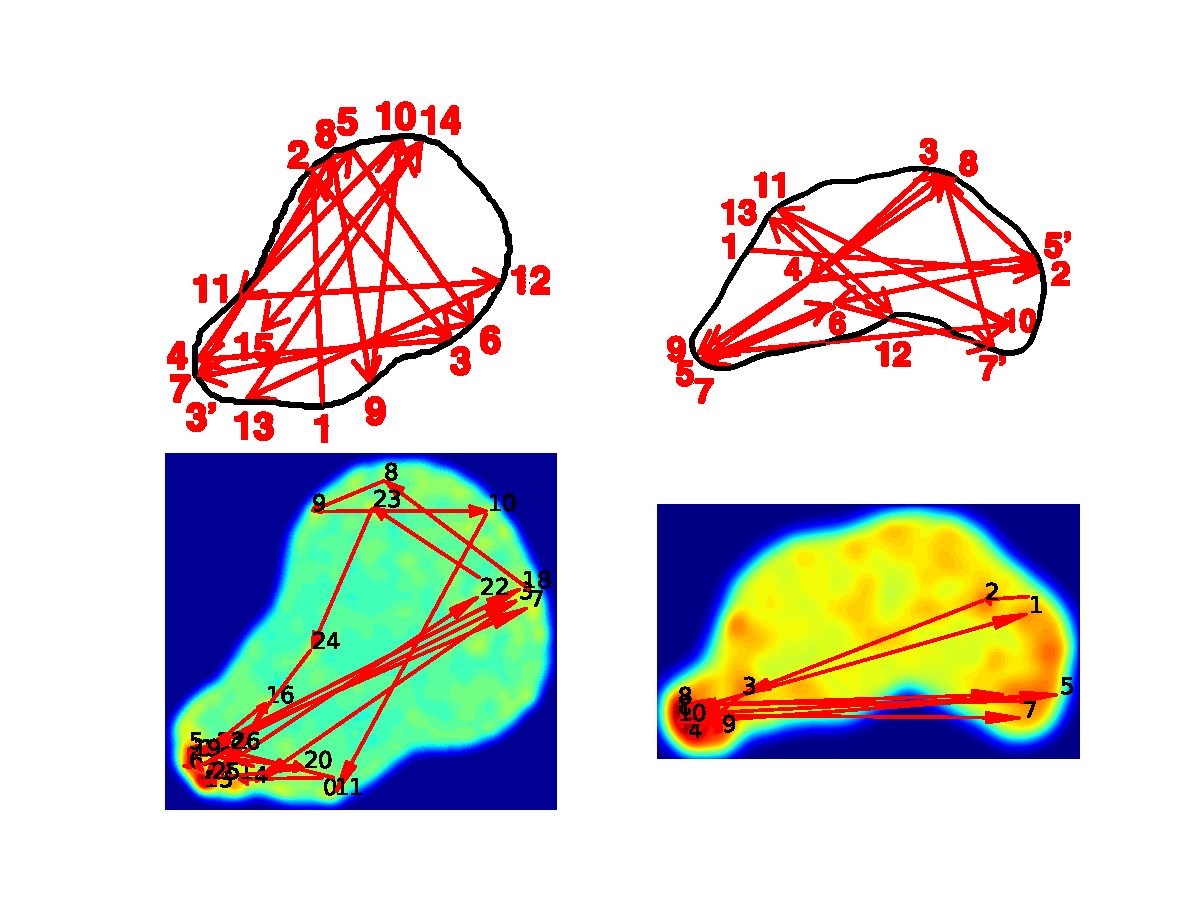
\includegraphics[width=0.8\textwidth]{../paper/plot-ave}
  \caption{We display here arrows depicting successive maxima in space
    and and time overlayed on a color plot of the total MinD density
    averaged over the same time period.  The simulation time covered
    for the flattened cells is \fixme{340} seconds, which is the same
    period of time depicted in the experimental data plots of Mannik
    \emph{et al.}~\cite{mannik2012robustness}.  For the wild type pill
    shape, we only cover \fixme{???} seconds, in order to provide a
    useful comparison due to its shorter oscillation period.  The top
    row shows plots published by Mannik of the MinD maxima behavoir
    and the bottom two rows show our simulations using the stochastic
    and deterministic models, respectively.  We simulated
    approximations to the two shapes observed by Mannik, which we call
    \emph{shape A} and \emph{shape B}.  In addition, we studied two
    flattened stadium shapes which we call \emph{stadium A} and
    \emph{stadium B} corresponding in aspect ratio and thickness to
    the two experimental shapes.  The spatial length scale of all the
    figures shown was identical. Each of the flattened cell shapes
    uses the same color scale for the number of proteins per unit
    area.  Finally, we display the natural pill shape, which was also
    featured in Figs.~\ref{image-p} and~\ref{corr-pill}, with a
    different color scale to reflect the thicker cell containing more
    proteins per cross-sectional area.  }
  \label{randst-plot-ave}
\end{figure*}

\section{Comparison of Mannik's Experimental and Our Stadium Shapes}

As describe in Section~\ref{sec:model-method-shapes}, we will focus on
simulation of four illustrative flattened cell shapes: two shapes
created to replicate those published by
Mannik~\cite{mannik2012robustness} (shape~\emph{A} and
shape~\emph{B}), and for comparison two symmetrical stadium shapes
that have the identical aspect ratio, thickness and volume (stadium
\emph{A} and stadium \emph{B}), shown in Figure~\ref{randst-plot-ave}.
These stadium shapes enable us to distinguish between the effect of
cellular shape irregularity and assymetry, and that of overall size
and aspect ratio.  We note that shape \emph{B} is more irregular than
shape \emph{A}, and in particular features a prominant region of
concavity on its left-hand side.  For each of these shapes (in
addition to the wild type pill shape discussed previously) we have
simulated in excess of \fixme{???}  seconds of evolution of the MinD
system using the deterministic version of Huang's
model~\cite{huang2003dynamic}, as well as the stochastic model.

From each of these flattened simulations, we have chosen a typical 350
second segment to compare with the results of Mannik exemplified in
arrow plots in which the arrow heads show the location of sequential
MinD maxima within the cell (over the same time
interval)~\cite{mannik2012robustness}.  In addition to arrows between
successive maxima in space and time, we plot as a colored background
the density of MinD protiens averaged over the same time period.  We
note that we have manually verified that our (computer-generated)
arrow plots also reflect a human interpretation of a movie of the same
data.  Finally, for comparison we present the same plot for a
wild-type cell, with a time period of \fixme{???}  seconds to account
for its short period of oscillation.

In every case, including the wild type pill shape, we see irregularity
in the location of the maxima when using the stochastic model.  The
deterministic model shows uniformly bipolar oscillation, with the
exception of shape \emph{B}, which develops weak intermediate maxima
on the right-hand edge of the cell.  From these results, we conclude
that the deterministic model is inadequate to explain experimental
observations of the locations of density maxima of the MinD protein.


%% We found that the deterministic simulations of the MinD system results
%% in robust and regular oscillatory behavoir of polar selection and
%% oscillation in not only symmetrical shapes, such as the wildtype pill
%% shape, but also in very assymetrical, flatttened cells, such as those
%% observed by Mannik.  We also examined larger and smaller versions of
%% these shapes, and found this behavior to be very robust, from the
%% minimum size to sustain oscillation (around \fixme{???} $\mu$m) up to
%% around twice the cell size reported by Mannik.  At larger sizes than
%% this, less regular oscillations occur using the deterministic method,
%% but we note that the cells reported by Mannik are already considerably
%% larger in volume than typical wild type
%% cells~\cite{kubitschek1990cell,kubitschek1968linear,mannik2012robustness}.

\begin{figure}
  \includegraphics[width=\columnwidth]{../data/shape-randst/0_25-18_50-18_50-95_00-15_00-full_array/plots/correlation.pdf}
  \includegraphics[width=\columnwidth]{../data/shape-stad/0_25-2_35-1_32-0_00-15_00-full_array/plots/correlation.pdf}
  \caption{Correlation for A shapes}
  \label{fig:corr-pancake-A}
\end{figure}

The predictions of the stochastic model as seen in
Fig.~\ref{randst-plot-ave} are roughly similar to the experimental
results in terms of irregularity of the locations of maxima, although
there are locations on the edges of the cells where experiment shows
maxima occuring that we never see in our simulations, suggesting that
the model does not precisely reflect the experiment.  We also note
that the stadium shapes in Fig.~\ref{randst-plot-ave} appear
qualitatively similar to the irregular shapes in terms of the
locations of their maxima.

However, Fig.~\ref{randst-plot-ave} leaves unclear the importance of
irregularity versus overall thickness and aspect ratio in developing
an understanding of the origin of the experimentally observed
behavior.  Although in the movies the stadiums appear to display a
more regular bipolar oscillation, the arrow plots do not provide a
convincing demonstration.  To illustrate the difference in behavior
between shape \emph{A} and stadium \emph{A}, we return in
Fig.~\ref{fig:corr-pancake-A} to the correlation function between the
number of proteins in a segment at the top of the cell and the number
of proteins in a segment at the bottom of the cell.  We computed these
correlation functions using over \fixme{???} seconds of simulation.
We found with the stochastic model that the experimental shape
\emph{A} has a coherence time of under 4 periods, while the
corresponding stadium \emph{A} has a coherence time of 10 periods.  In
each case, the deterministic model is perfectly periodic. This
confirms that with the stochastic model the stadium shape does indeed
have a far more regular bipolar oscillation than the irregular shape
\emph{A}.  When we compare shape \emph{B} and stadium \emph{B}, we see
a similar effect, although both coherence times are somewhat smaller
(2.7 and 6.2, respectively).  From these results we conclude that the
irregularity seen experimentally is indeed exacerbated by the
irregular shapes taken on by the cells forced into a thin slit.

\section{Conclusion}
We have simulated flattened cell shapes similar to those observed
experimentally by Mannik \emph{et al.}.  We find that the
deterministic model~\fixme{cite} predicts behavior that completely
contradicts what is seen experimentally: it predicts stable and
periodic bipolar oscillation, with a minor intermediate maximum
appearing in shape \emph{B}.  Thus we conclude that this method is
inconsistent with experiment, and should not be relied upon for
predictions of the behavior of the MinD system.

As found in previous studies~\fixme{cite}, we observe that the
stochastic model predicts behavior in wild type cells that is
consistent both with experiment and with the deterministic model.  In
contrast, the stochastic model~\fixme{cite} predicts spatially
irregular formation of maxima for all the flattened cells that we
studied.  In order to better understand the irregular oscillations
observed in experiment, we simulated flattened ``stadium'' shapes in
order to distinguish between the effect of flattening and the effect
of irregular shape.  We found that although the stadium cells
exhibited somewhat more irregular locations of maxima than the
wild-type cells, their oscillation was far more periodic and bipolar
than the irregular cell shapes observed experimentally.  Thus we
confirm that the disruption of the MinD oscillations seen by Mannik
\emph{et al.} is largely due to the irregularity of cell shapes
observed, as opposed to the size or aspect ratio.

\bibliography{paper}

\begin{figure}
  \includegraphics[width=\columnwidth]{../data/shape-randst/0_25-18_60-28_60-94_00-15_00-full_array/plots/correlation.pdf}
  \includegraphics[width=\columnwidth]{../data/shape-stad/0_25-2_92-1_18-0_00-15_00-full_array/plots/correlation.pdf}
  \caption{Correlation for B shapes}
  \label{corr-B}
\end{figure}

\end{document}

\section*{Appendix}

\section{Below are NOTES for the Writing}


\end{document}
